\documentclass[10pt,a4paper,twoside]{article}

% \usepackage[margin=2cm]{geometry}
\usepackage[inner=2.5cm,outer=1.5cm,top=1.5cm,bottom=1.5cm]{geometry}
\usepackage{fontspec}
% \usepackage{mathptmx}
\usepackage{contour}
\usepackage[none]{hyphenat}
\setmainfont{Comic Sans MS}
\usepackage[dvipsnames]{xcolor}
\usepackage{graphicx}
\usepackage{tikz}
\usetikzlibrary{shapes.callouts,positioning}
\usepackage[pages=some,placement=top]{background}

\newcommand{\englang}[1]{
    #1 %comment/uncomment this line to hide/show english
}
\newcommand{\italang}[1]{
    % #1 %comment/uncomment this line to hide/show italian
}

% \renewcommand*\familydefault{\sfdefault}

% \pagenumbering{gobble}
\graphicspath{{./figures/}}

\englang{
\title{\fontsize{52}{62}\selectfont \contour{black}{\textcolor{white}{\textbf{ECHOES OF HOPE}}}}
\author{\fontsize{20}{30}\selectfont \contour{black}{\textcolor{white}{\textbf{A JOURNEY BEYOND THE STARS}}}}
\date{}
}

\italang{
\title{\fontsize{45}{56}\selectfont \contour{black}{\textcolor{white}{\textbf{ECHI DI SPERANZA}}}}
\author{\fontsize{20}{30}\selectfont \contour{black}{\textcolor{white}{\textbf{UN VIAGGIO OLTRE LE STELLE}}}}
\date{}
}



\begin{document}

\maketitle

~
\backgroundsetup{
scale=1.1,
angle=0,
opacity=1,  %% adjust
contents={
\includegraphics[keepaspectratio]{cover}}
}
\BgThispage
\thispagestyle{empty}

\vfill
\hfill
{\Large \contour{black}{\textcolor{white}{\textbf{Lara Vignotto}}}}

\newpage
~
\newpage



%%%%%%%%%% PAGE 1
\noindent
\begin{minipage}{1.4\textwidth}
    \vspace{1cm}
    \begin{tikzpicture}
        \node (img) {\frame{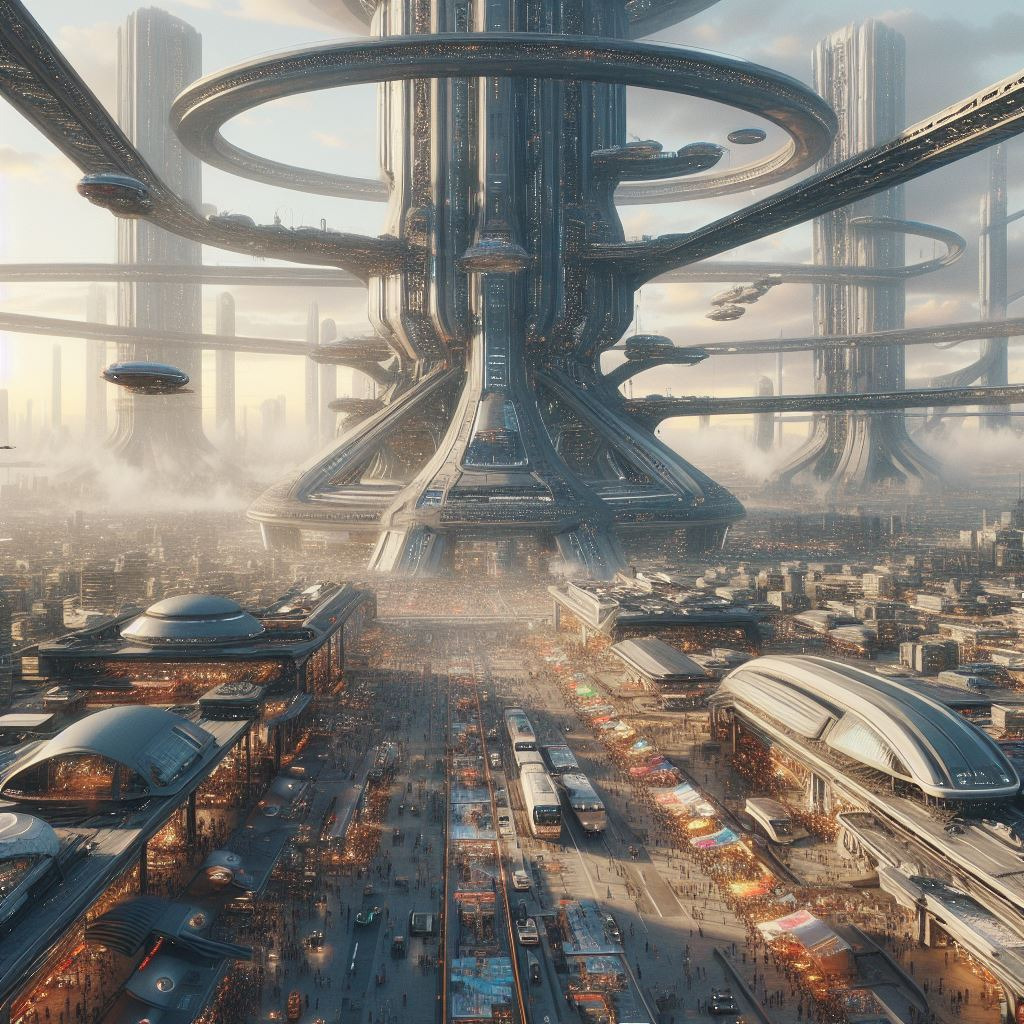
\includegraphics[width=\textwidth]{p1s1}}};
        \node [text width=5cm, align=center, rectangle callout, fill=white, draw, callout relative pointer={(0,0)}] at (-8,10) {
            \englang{SANCTUM PRIME: A HEAVEN BEYOND EARTH}
            \italang{SANCTUM PRIME:\\UN PARADISO OLTRE LA TERRA}
            };
        \node [text width=7cm, align=center, rectangle callout, fill=white, draw, callout relative pointer={(0,0)}] at (2.5,6) {
            \englang{AN ARCOLOGY, LIKE SANCTUM PRIME, STANDS AS A SELF-SUSTAINING OASIS BEYOND EARTH---A TOWERING CITYSCAPE WHERE HUMANITY THRIVES AMIDST THE EXPANSE OF DEEP SPACE, A TESTAMENT TO HUMAN RESILIENCE AND INNOVATION}
            \italang{UN'ARCOLOGIA, COME SANCTUM PRIME, SI ERGE COME UN'OASI AUTOSUFFICIENTE AL DI LÀ DELLA TERRA---UN PAESAGGIO URBANO VERTIGINOSO DOVE L'UMANITÀ PROSPERA NELL'IMMENSITÀ DELLO SPAZIO PROFONDO, UNA TESTIMONIANZA DELLA RESILIENZA E DELL'INNOVAZIONE UMANA}
            };
        \node [text width=6.5cm, align=center, rectangle callout, fill=white, draw, callout relative pointer={(0,0)}] at (-6.5,-7.5) {
            \englang{ARCOLOGIES ARE VERTICAL CITIES, WHERE PEOPLE LIVE, WORK, AND CREATE WITHIN TOWERING STRUCTURES, A MICROCOSM OF CIVILIZATION SUSTAINED BY ADVANCED TECHNOLOGY, PROVIDING SHELTER, RESOURCES, AND COMMUNITY IN THE VASTNESS OF SPACE}
            \italang{LE ARCOLOGIE SONO CITTÀ VERTICALI, DOVE LE PERSONE VIVONO, LAVORANO, E CREANO ALL'INTERNO DI STRUTTURE IMPONENTI, UN MICROCOSMO DI CIVILTÀ SOSTENUTO DA TECNOLOGIE AVANZATE, CHE FORNISCONO RIPARO, RISORSE E COMUNITÀ NELLA VASTITÀ DELLO SPAZIO}
            };
    \end{tikzpicture}
\end{minipage}%

\newpage



%%%%%%%%%% PAGE 2
\noindent
\begin{minipage}{0.49\textwidth}
    \begin{tikzpicture}
        \node (img) {\frame{
\includegraphics[width=\textwidth]{p2s1}}};
        \node [text width=5cm, align=center, rectangle callout, fill=white, draw, callout relative pointer={(0,0)}] at (-1,4) {
            \englang{DR.~EVELYN HAYES, COMMUNICATION SCIENTIST}
            \italang{DOTT.SSA EVELYN HAYES, SCIENZIATA DELLA COMUNICAZIONE}
            };
        \node [text width=2.5cm, align=center, ellipse callout, fill=white, draw, callout relative pointer={(0.5,0.5)}] at (-2,-2.5) {
            \englang{THE SIGNAL PATTERNS ARE PERSISTENT, LILY}
            \italang{I MODELLI DI SEGNALE SONO PERSISTENTI, LILY.}
            };
        \node [text width=2.5cm, align=center, ellipse callout, fill=white, draw, callout relative pointer={(-0.5,1)}] at (2,-3.2) {
            \englang{WHAT DO YOU SEE UP THERE, LILY?}
            \italang{COSA VEDI LASSU, LILY?}
            };
    \end{tikzpicture}
\end{minipage}%
\hfill
\begin{minipage}{0.49\textwidth}
    \italang{\vspace{0.4cm}}
    \begin{tikzpicture}
        \node (img) {\frame{
\includegraphics[width=\textwidth]{p2s2}}};
    \end{tikzpicture}
\end{minipage}%
\vspace{.1cm}
\noindent\hspace{1pt}
\begin{minipage}{1\textwidth}
    \begin{tikzpicture}
        \node (img) {\frame{
\includegraphics[width=\textwidth]{p2s3}}};
        \node [dashed, text width=3cm, align=center, ellipse callout, fill=white, draw, callout relative pointer={(0,0)}] at (5,5) {
            \englang{THEY WANT US TO HEAR THEM.}
            \italang{VOGLIONO CHE LI ASCOLTIAMO.}
            };
        \draw [dashed, fill=white, draw] (4.5,3.5) ellipse (.5cm and .25cm);
        \draw [dashed, fill=white, draw] (3.8,2.8) ellipse (.25cm and .125cm);
    \end{tikzpicture}
\end{minipage}%

\newpage



%%%%%%%%%% PAGE 3
~\vspace{0.8cm}

\noindent
\begin{minipage}{0.49\textwidth}
    \vspace{0.7cm}
    \begin{tikzpicture}
        \node (img) {\frame{
\includegraphics[width=\textwidth]{p3s1}}};
        \node [text width=4.5cm, align=center, ellipse callout, fill=white, draw, callout relative pointer={(-0.1,1)}] at (-.5,-5) {
            \englang{THE SIGNAL PATTERNS ARE PERSISTENT, BUT THEIR ORIGIN REMAINS ELUSIVE...}
            \italang{GLI SCHEMI DEL SEGNALE SONO PERSISTENTI, MA LA LORO ORIGINE SEMBRA SFUGGENTE...}
            };
    \end{tikzpicture}
\end{minipage}%
\hfill
\begin{minipage}{0.49\textwidth}
    \begin{tikzpicture}
        \node (img) {\frame{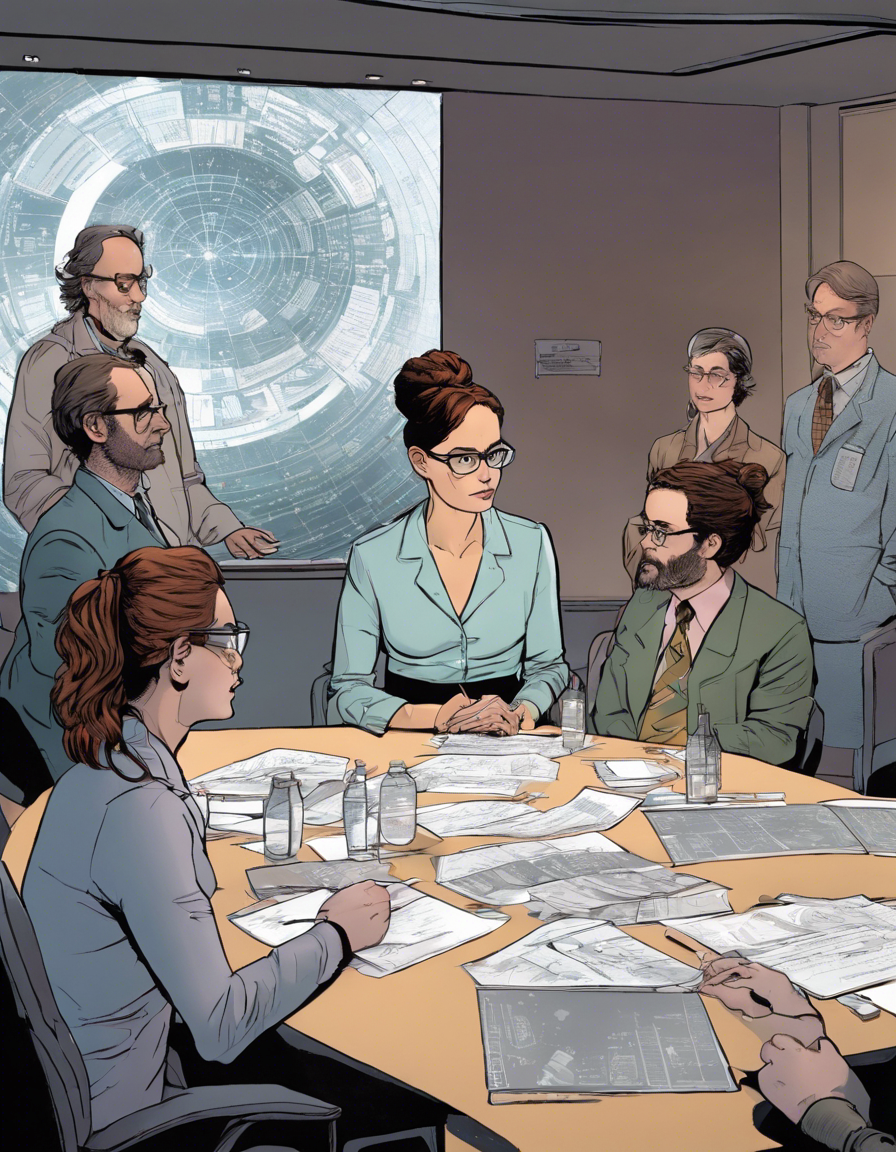
\includegraphics[width=\textwidth]{p3s2}}};
        \node [text width=4.5cm, align=center, ellipse callout, fill=white, draw, callout relative pointer={(-0.5,1.2)}] at (0,-4) {
            \englang{OUR SITUATION IS CRITICAL. WE MUST FIND SOLUTIONS BEFORE IT'S TOO LATE!}
            \italang{
                LA NOSTRA SITUAZIONE È CRITICA. DOBBIAMO TROVARE DELLE SOLUZIONI PRIMA CHE SIA TROPPO TARDI!}
            };
        \node [text width=3.5cm, align=center, rectangle callout, fill=white, draw, callout relative pointer={(0,0)}] at (1.8,4.5) {
            \englang{IN THE MEETING ROOM}
            \italang{NELLA SALA CONFERENZE}
            };
    \end{tikzpicture}
\end{minipage}%
\vspace{0.5cm}
\noindent\hspace{1pt}
\begin{minipage}{0.49\textwidth}
    \vspace{0.85cm}
    \italang{\vspace{0.6cm}}
    \begin{tikzpicture}
        \node (img) {\frame{
\includegraphics[width=\textwidth]{p3s3}}};
        \node [text width=3.5cm, align=center, rectangle callout, fill=white, draw, callout relative pointer={(0,0)}] at (-1.8,3.2) {
            \englang{BACK IN THE QUARTERS}
            \italang{NEGLI ALLOGGI}
            };
        \node [dashed, text width=2.5cm, align=center, ellipse callout, fill=white, draw, callout relative pointer={(0,0)}] at (-2,-3.5) {
            \englang{THEY'RE ASKING FOR HELP. I CAN FEEL IT.}
            \italang{STANNO CHIEDENDO AIUTO. LO SENTO.}
            };
        \draw [dashed, fill=white, draw] (-2.2,-1.1) ellipse (.5cm and .25cm);
        \draw [dashed, fill=white, draw] (-1.8,-0.6) ellipse (.25cm and .125cm);
    \end{tikzpicture}
\end{minipage}%
\hfill
\begin{minipage}{0.49\textwidth}
    \begin{tikzpicture}
        \node (img) {\frame{
\includegraphics[width=\textwidth]{p3s4}}};
        \node [text width=2.5cm, align=center, ellipse callout, fill=white, draw, callout relative pointer={(-0.5,-0.5)}] at (2,3) {
            \englang{LILY, YOU SHOULDN'T BE SEEING THIS. IT'S NOT SAFE.}
            \italang{LILY, NON DOVRESTI VEDERE TUTTO QUESTO. NON È SICURO.}
            };
    \end{tikzpicture}
\end{minipage}%

\newpage



%%%%%%%%%% PAGE 4
~\vspace{1cm}

\noindent
\begin{minipage}{0.49\textwidth}
    \begin{tikzpicture}
        \node (img) {\frame{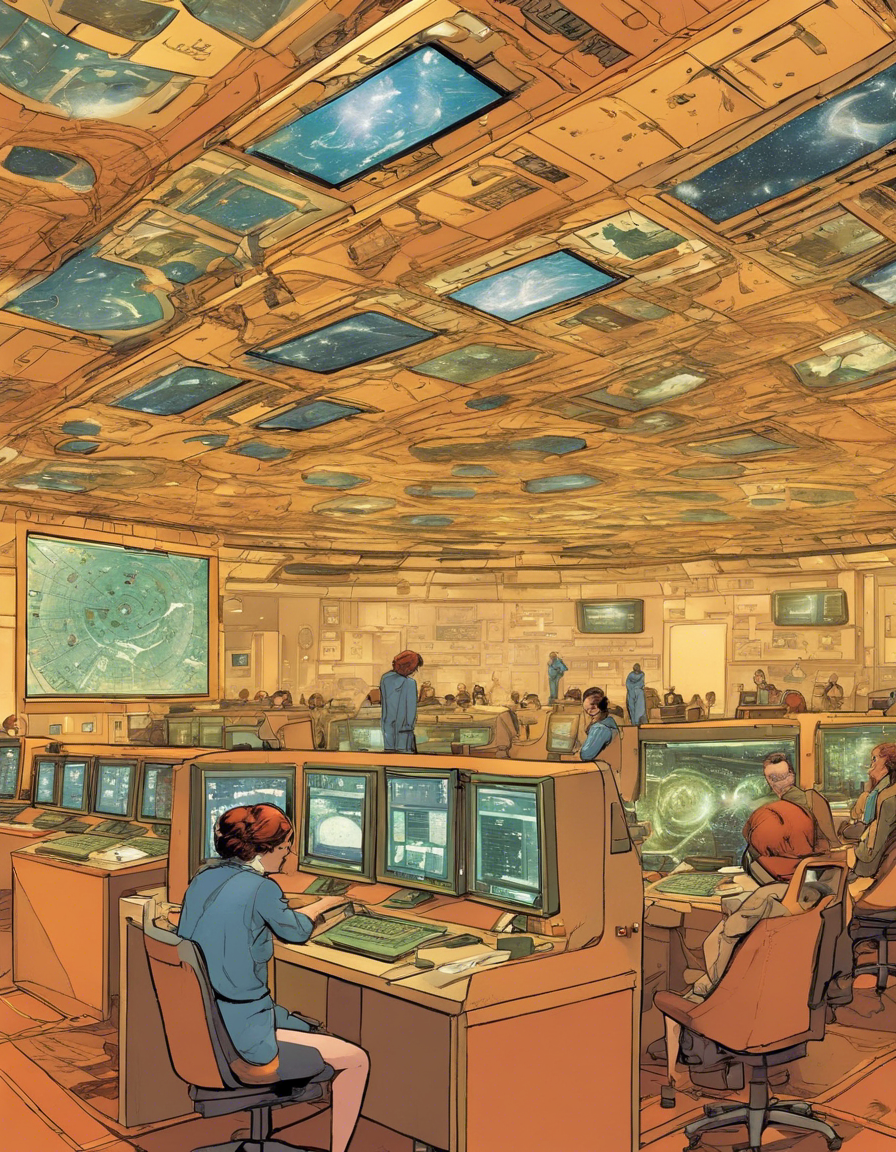
\includegraphics[width=\textwidth]{p4s1}}};
        \node [text width=3.5cm, align=center, rectangle callout, fill=white, draw, callout relative pointer={(0,0)}] at (-1.8,4.5) {
            \englang{IN THE COMMUNICATION STATION}
            \italang{NELLA STAZIONE DI COMUNICAZIONE}
            };
        \node [text width=4.5cm, align=center, ellipse callout, fill=white, draw, callout relative pointer={(0,-1)}] at (0.5,2.5) {
            \englang{WHAT'S HAPPENING? THIS IS UNPRECEDENTED!}
            \italang{COSA STA SUCCEDENDO? È SENZA PRECEDENTI!}
            };
    \end{tikzpicture}
\end{minipage}%
\hfill
\begin{minipage}{0.49\textwidth}
    \begin{tikzpicture}
        \node (img) {\frame{
\includegraphics[width=\textwidth]{p4s2}}};
        \node [text width=4cm, align=center, ellipse callout, fill=white, draw, callout relative pointer={(-0.5,-1)}] at (1,4.5) {
            \englang{THIS SIGNAL---IT'S A CRY FOR HELP!}
            \italang{QUESTO SEGNALE---È UN GRIDO D'AIUTO!}
            };
    \end{tikzpicture}
\end{minipage}%
\vspace{0.2cm}
\noindent\hspace{1pt}
\begin{minipage}{0.49\textwidth}
    \begin{tikzpicture}
        \node (img) {\frame{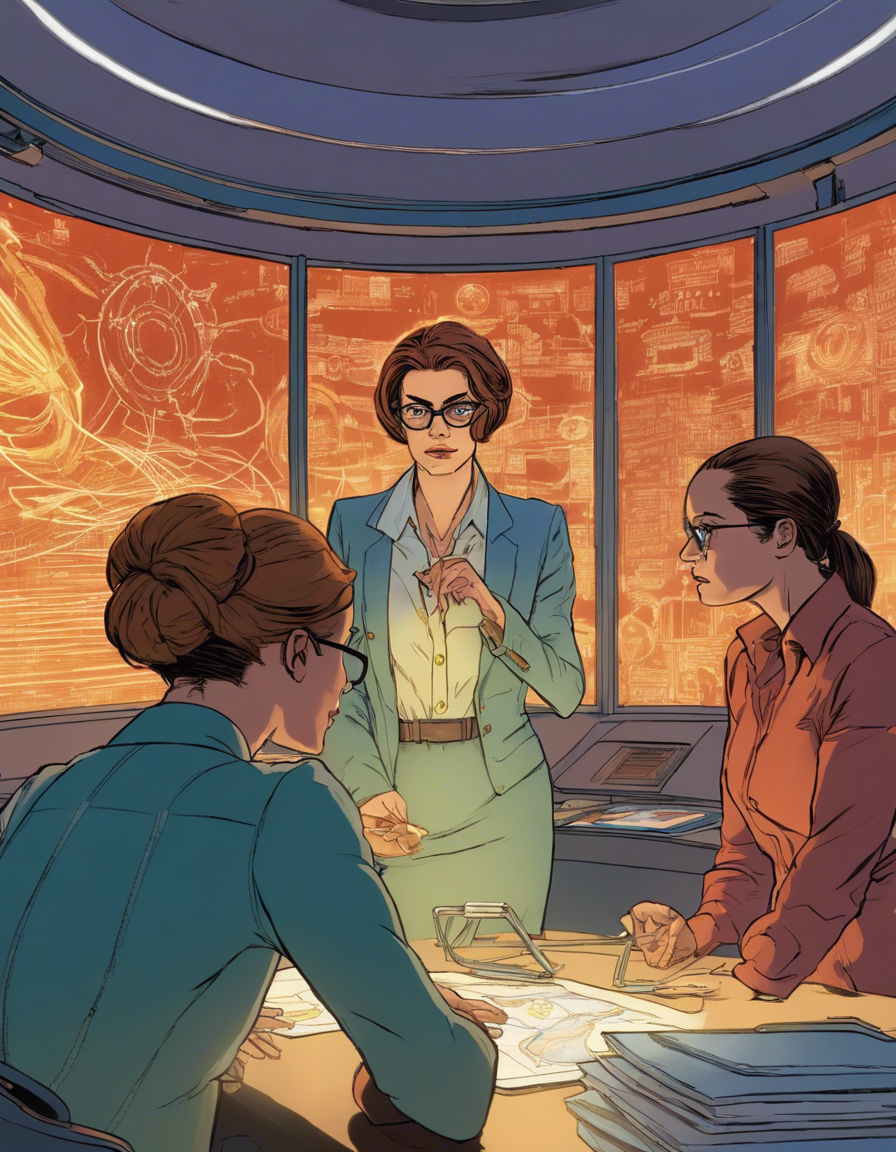
\includegraphics[width=\textwidth]{p4s3}}};
        \node [text width=3cm, align=center, ellipse callout, fill=white, draw, callout relative pointer={(0.2,-0.5)}] at (-1.8,3.5) {
            \englang{WE NEED TO ACT FAST! LIVES MAY BE AT STAKE!}
            \italang{DOBBIAMO AGIRE VELOCEMENTE! DELLE VITE POTREBBERO ESSERE IN PERICOLO!}
            };
    \end{tikzpicture}
\end{minipage}%
\hfill
\begin{minipage}{0.49\textwidth}
    \vspace{2.05cm}
    \italang{\vspace{0.6cm}}
    \begin{tikzpicture}
        \node (img) {\frame{
\includegraphics[width=\textwidth]{p4s4}}};
        \node [text width=5cm, align=center, ellipse callout, fill=white, draw, callout relative pointer={(0,1)}] at (0,-4.2) {
            \englang{PREPARE THE EXPEDITION. WE'RE GOING TO INVESTIGATE THE SOURCE OF THIS SIGNAL OURSELVES.}
            \italang{PREPARATE L'ESPLORAZIONE. È ORA DI INDAGARE SULLA FONTE DI QUESTO SEGNALE.}
            };
    \end{tikzpicture}
\end{minipage}%

\newpage 



%%%%%%%%%% PAGE 5
~\vspace{1.5cm}

\noindent
\begin{minipage}{0.49\textwidth}
    \begin{tikzpicture}
        \node (img) {\frame{
\includegraphics[width=\textwidth]{p5s1}}};
        \node [text width=2cm, align=center, ellipse callout, fill=white, draw, callout relative pointer={(0,-1)}] at (2.5,1.2) {
            \englang{THEY'RE SCARED. I CAN FEEL IT.}
            \italang{HANNO PAURA. LO SENTO.}
            };
    \end{tikzpicture}
\end{minipage}%
\hfill
\begin{minipage}{0.49\textwidth}
    \italang{\vspace{0.6cm}}
    \begin{tikzpicture}
        \node (img) {\frame{
\includegraphics[width=\textwidth]{p5s2}}};
        \node [text width=2.5cm, align=center, ellipse callout, fill=white, draw, callout relative pointer={(0,0.5)}] at (-2,-2.5) {
            \englang{LILY, YOU SHOULDN'T BE SEEING THIS. IT'S NOT SAFE.}
            \italang{LILY, NON DOVRESTI VEDERE TUTTO QUESTO. NON È SICURO.}
            };
    \end{tikzpicture}
\end{minipage}%
\vspace{2.3cm}
\noindent\hspace{1pt}
\begin{minipage}{0.49\textwidth}
    \begin{tikzpicture}
        \node (img) {\frame{
\includegraphics[width=\textwidth]{p5s3}}};
        \node [text width=2cm, align=center, ellipse callout, fill=white, draw, callout relative pointer={(0.5,0)}] at (-2.6,0.8) {
            \englang{THEY'RE ASKING FOR HELP. WE HAVE TO DO SOME- THING.}
            \italang{STANNO CHIEDENDO AIUTO. DOBBIAMO FARE QUALCOSA.}
            };
    \end{tikzpicture}
\end{minipage}%
\hfill
\begin{minipage}{0.49\textwidth}
    \vspace{1.15cm}
    \italang{\vspace{0.2cm}}
    \begin{tikzpicture}
        \node (img) {\frame{
\includegraphics[width=\textwidth]{p5s4}}};
        \node [dashed, text width=2.5cm, align=center, ellipse callout, fill=white, draw, callout relative pointer={(0,0)}] at (-2.2,3.5) {
            \englang{PERHAPS LILY HOLDS THE KEY TO UNLOCKING THE MYSTERY BEHIND THIS SIGNAL.}
            \italang{FORSE LILY È LA CHIAVE PER SCOPRIRE IL MISTERO DI QUESTO SEGNALE.}
            };
        \draw [dashed, fill=white, draw] (0.3,4.3) ellipse (.5cm and .25cm);
        \draw [dashed, fill=white, draw] (0.8,3.8) ellipse (.25cm and .125cm);
    \end{tikzpicture}
\end{minipage}%

\newpage 



%%%%%%%%%% PAGE 6
~\vspace{0.8cm}

\noindent
\begin{minipage}{0.49\textwidth}
    \vspace{0.8cm}
    \italang{\vspace{0.6cm}}
    \begin{tikzpicture}
        \node (img) {\frame{
\includegraphics[width=\textwidth]{p6s1}}};
        \node [dashed, text width=3cm, align=center, ellipse callout, fill=white, draw, callout relative pointer={(0,0)}] at (-1.5,-3) {
            \englang{HOW DOES SHE UNDERSTAND?}
            \italang{COME FA A CAPIRE?}
            };
        \draw [dashed, fill=white, draw] (-2.2,-1.6) ellipse (.5cm and .25cm);
        \draw [dashed, fill=white, draw] (-2,-0.8) ellipse (.25cm and .125cm);
    \end{tikzpicture}
\end{minipage}%
\hfill
\begin{minipage}{0.49\textwidth}
    \begin{tikzpicture}
        \node (img) {\frame{
\includegraphics[width=\textwidth]{p6s2}}};
        \node [text width=2.7cm, align=center, ellipse callout, fill=white, draw, callout relative pointer={(-0.3,-0.5)}] at (2,3.5) {
            \englang{WE NEED TO UNITE OUR EXPERTISE. OUR MISSION IS CLEAR.}
            \italang{DOBBIAMO UNIRE LE NOSTRE COMPETENZE. LA NOSTRA MISSIONE È CHIARA.}
            };
    \end{tikzpicture}
\end{minipage}%
\vspace{1cm}
\noindent\hspace{1pt}
\begin{minipage}{0.49\textwidth}
    \vspace{3.1cm}
    \italang{\vspace{0.3cm}}
    \begin{tikzpicture}
        \node (img) {\frame{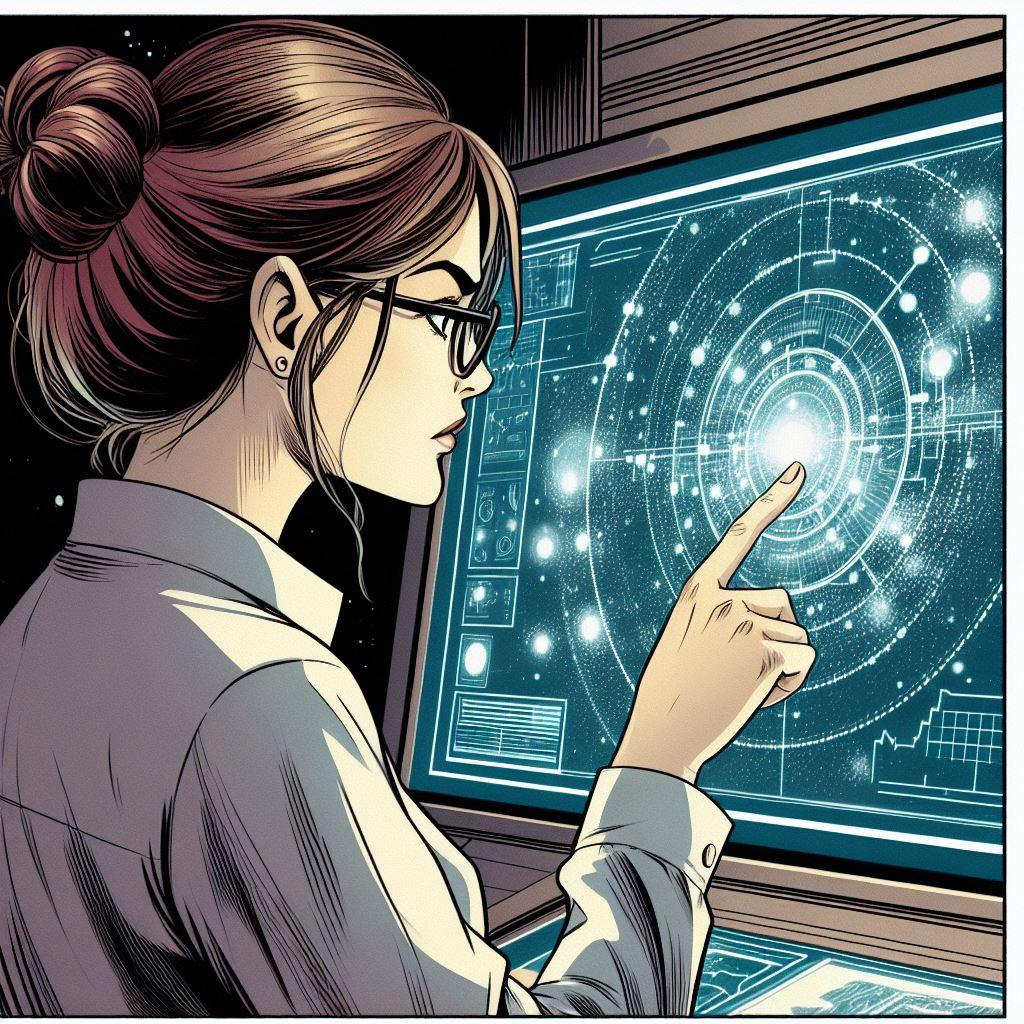
\includegraphics[width=\textwidth]{p6s3}}};
        \node [text width=4cm, align=center, ellipse callout, fill=white, draw, callout relative pointer={(0,0.5)}] at (-1,-3.5) {
            \englang{OUR DESTINATION LIES BEYOND THE ARCOLOGY'S REACH. BUT WE MUST GO WHERE THE SIGNAL LEADS US.}
            \italang{LA NOSTRA DESTINAZIONE È AL DI LÀ DELLA PORTATA DELL'ARCOLOGIA. MA DOBBIAMO ANDARE DOVE CI PORTA IL SEGNALE.}
            };
    \end{tikzpicture}
\end{minipage}%
\hfill
\begin{minipage}{0.49\textwidth}
    \begin{tikzpicture}
        \node (img) {\frame{
\includegraphics[width=\textwidth]{p6s4}}};
        \node [text width=5cm, align=center, ellipse callout, fill=white, draw, callout relative pointer={(0,1)}] at (0,-5.5) {
            \englang{WE CANNOT IGNORE THEIR CALL. OUR JOURNEY BEGINS NOW.}
            \italang{NON POSSIAMO IGNORARE IL LORO APPELLO. IL NOSTRO VIAGGIO INIZIA ORA.}
            };
    \end{tikzpicture}
\end{minipage}%

\newpage 



%%%%%%%%%% PAGE 7
% ~\vspace{2cm}

\noindent
\begin{minipage}{0.75\textwidth}
    \hspace{1.37cm}
    \begin{tikzpicture}
        \node (img) {\frame{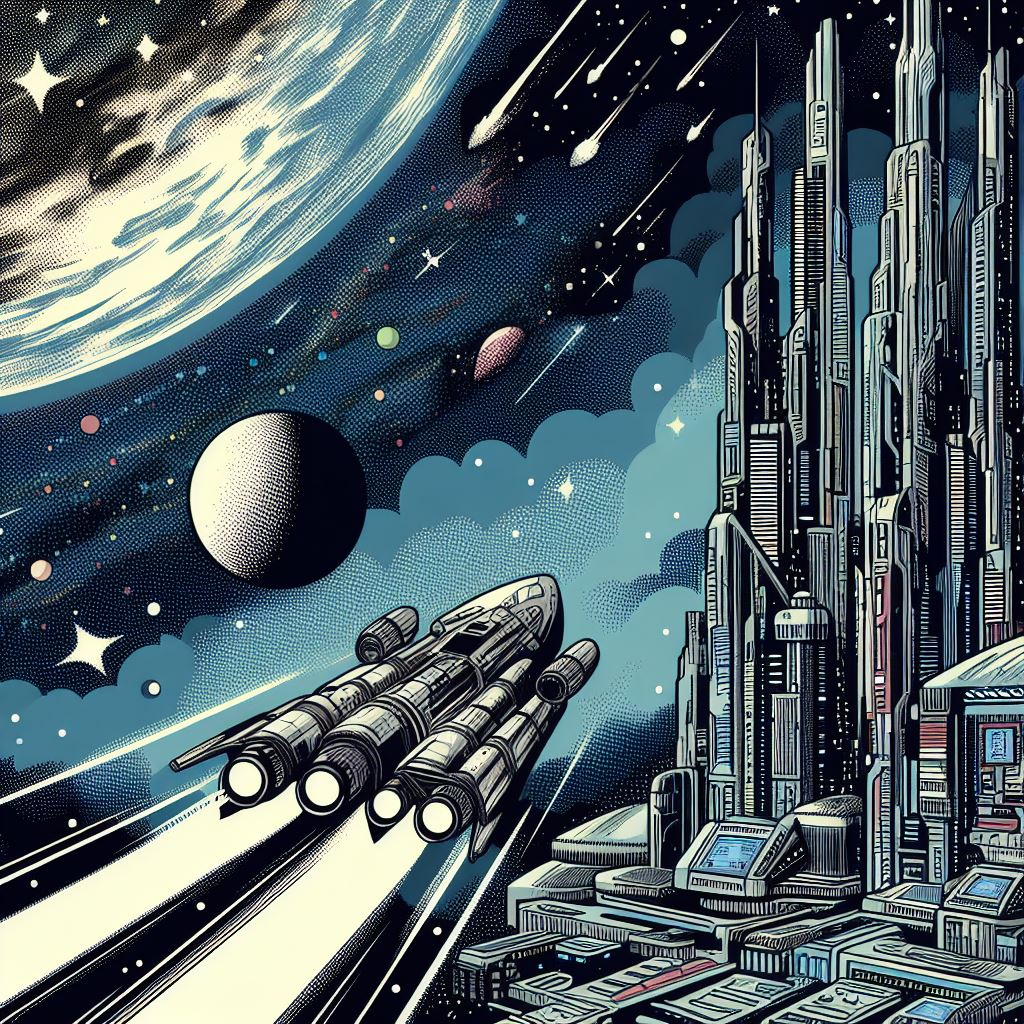
\includegraphics[width=\textwidth]{p7s1}}};
        \node [text width=5cm, align=center, rectangle callout, fill=white, draw, callout relative pointer={(0,0)}] at (-4.5,3.5) {
            \englang{WE'RE HEADING INTO THE UNKNOWN. BUT WE MUST GO WHERE THE SIGNAL LEADS US.}
            \italang{CI STIAMO INOLTRANDO NELL'IGNOTO. MA DOBBIAMO ANDARE DOVE CI PORTA IL SEGNALE.}
            };
    \end{tikzpicture}
\end{minipage}%

\vspace{0.2cm}

\noindent%\hspace{1pt}
\begin{minipage}{0.75\textwidth}
    \hspace{2cm}
    \begin{tikzpicture}
        \node (img) {\frame{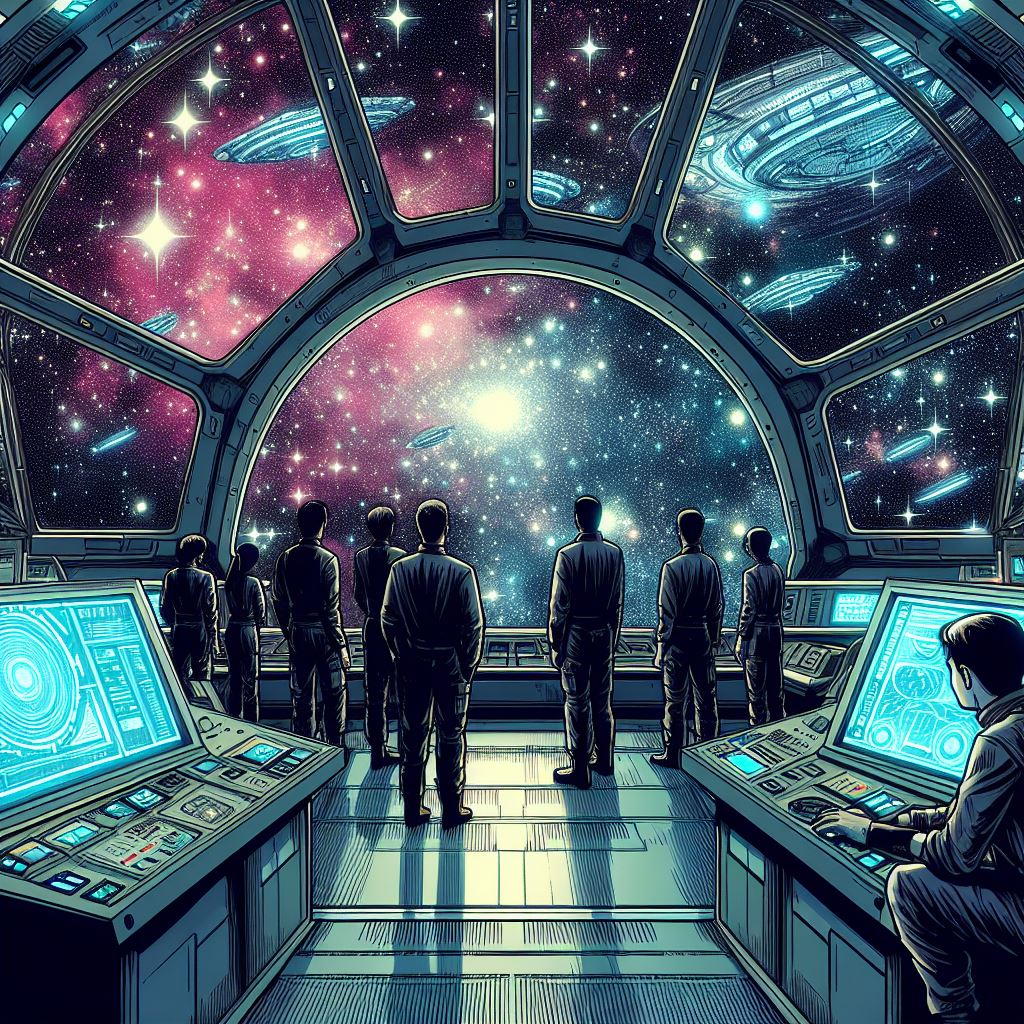
\includegraphics[width=\textwidth]{p7s2}}};
        \node [text width=5cm, align=center, ellipse callout, fill=white, draw, callout relative pointer={(-1,-0.5)}] at (4.5,2.5) {
            \englang{THIS IS BEYOND ANYTHING WE IMAGINED! BUT WE'RE READY FOR WHATEVER LIES AHEAD.}
            \italang{QUESTO VA OLTRE OGNI IMMAGINAZIONE! MA SIAMO PRONTI A TUTTO.}
            };
    \end{tikzpicture}
\end{minipage}%

\newpage 



%%%%%%%%%% PAGE 8
\noindent
\begin{minipage}{0.49\textwidth}
    \begin{tikzpicture}
        \node (img) {\frame{
\includegraphics[width=\textwidth]{p8s1}}};
        \node [text width=4cm, align=center, ellipse callout, fill=white, draw, callout relative pointer={(-0.2,-0.4)}] at (1.1,3) {
            \englang{WE CANNOT FALTER. LIVES MAY DEPEND ON OUR SUCCESS.}
            \italang{NON POSSIAMO VACILLARE. DELLE VITE POTREBBERO DIPENDERE DAL NOSTRO SUCCESSO.}
            };
    \end{tikzpicture}
\end{minipage}%
\hfill
\begin{minipage}{0.49\textwidth}
    \italang{\vspace{0.3cm}}
    \begin{tikzpicture}
        \node (img) {\frame{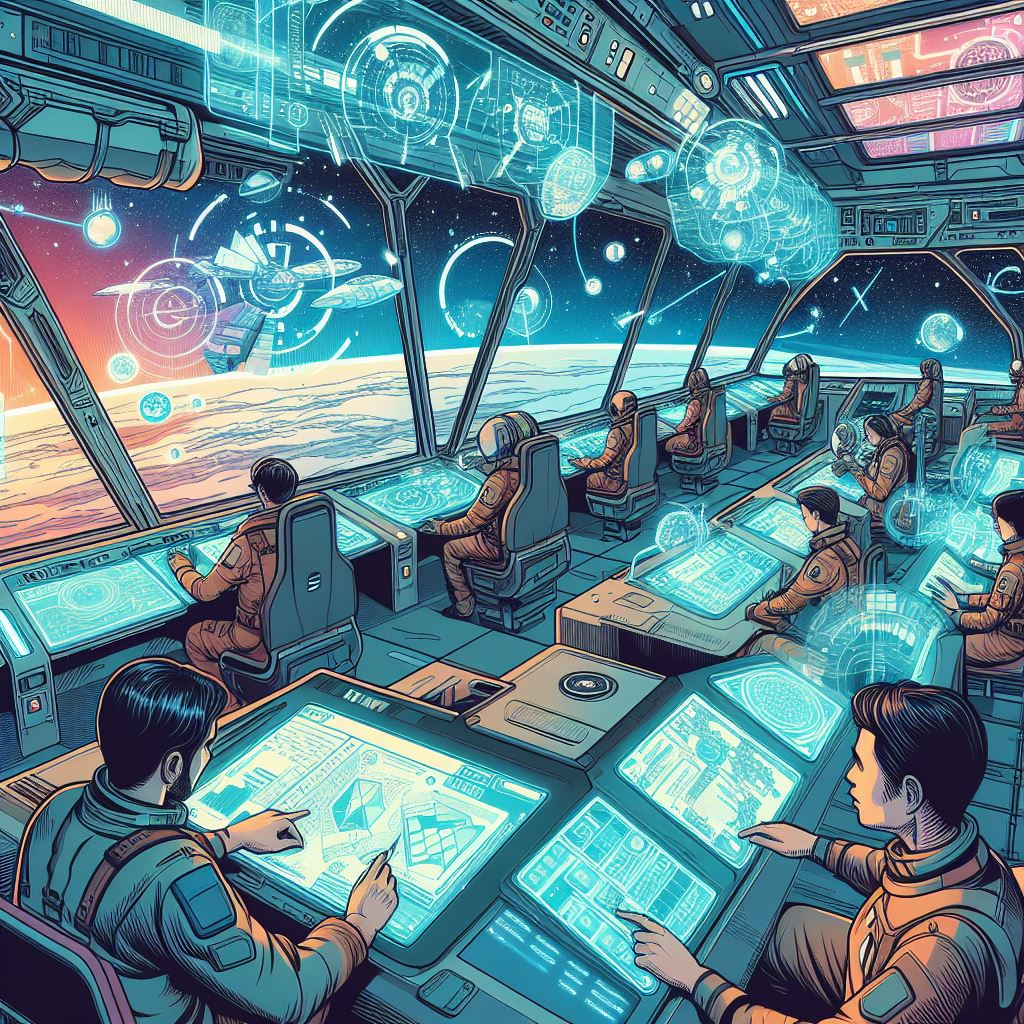
\includegraphics[width=\textwidth]{p8s2}}};
        \node [text width=3.5cm, align=center, ellipse callout, fill=white, draw, callout relative pointer={(0,0)}] at (-1.5,-2.8) {
            \englang{WE'RE MAKING PROGRESS! BUT WE MUST REMAIN VIGILANT.}
            \italang{STIAMO FACENDO PROGRESSI! MA DOBBIAMO RIMANERE VIGILI.}
            };
    \end{tikzpicture}
\end{minipage}%
\vspace{.1cm}
\noindent\hspace{1pt}
\begin{minipage}{1\textwidth}
    \begin{tikzpicture}
        \node (img) {\frame{
\includegraphics[width=\textwidth]{p8s3}}};
        \node [text width=4.5cm, align=center, ellipse callout, fill=white, draw, callout relative pointer={(0,0)}] at (4,6) {
            \englang{OUR JOURNEY HAS JUST BEGUN. BUT WE WILL NOT REST UNTIL WE HAVE ANSWERS.}
            \italang{IL NOSTRO VIAGGIO È APPENA INIZIATO. MA NON CI RIPOSEREMO FINCHÉ NON AVREMO RISPOSTE.}
            };
    \end{tikzpicture}
\end{minipage}%

\newpage



%%%%%%%%%% PAGE 9
~\vspace{0.6cm}

\noindent
\begin{minipage}{0.49\textwidth}
    \italang{\vspace{0.6cm}}
    \begin{tikzpicture}
        \node (img) {\frame{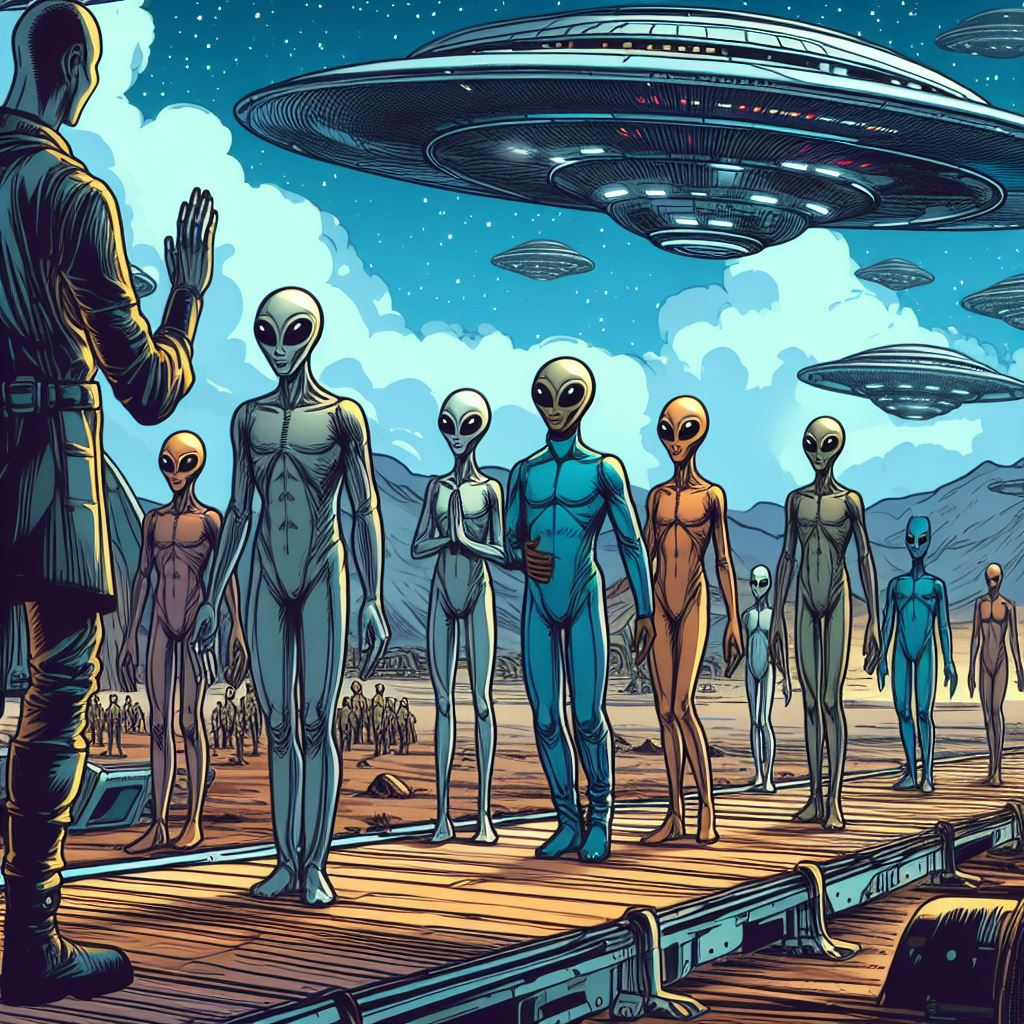
\includegraphics[width=\textwidth]{p9s1}}};
        \node [text width=5cm, align=center, rectangle callout, fill=white, draw, callout relative pointer={(0,0)}] at (-1,3.2) {
            \englang{THE SPACESHIP DOCKS AT AN ALIEN OUTPOST}
            \italang{L'ASTRONAVE ATTERRA SU UN AVAMPOSTO ALIENO}
            };
        \node [text width=3.5cm, align=center, ellipse callout, fill=white, draw, callout relative pointer={(0.5,0.8)}] at (-1,-3.5) {
            \englang{WELCOME TRAVELERS. WE ARE HONORED BY YOUR PRESENCE.}
            \italang{BENVENUTI VIAGGIATORI. SIAMO ONORATI DALLA VOSTRA PRESENZA.}
            };
    \end{tikzpicture}
\end{minipage}%
\hfill
\begin{minipage}{0.49\textwidth}
    \vspace{0.4cm}
    \begin{tikzpicture}
        \node (img) {\frame{
\includegraphics[width=\textwidth]{p9s2}}};
        \node [text width=5cm, align=center, ellipse callout, fill=white, draw, callout relative pointer={(-0.5,1)}] at (0,-3.5) {
            \englang{WE ARE HERE TO OFFER OUR ASSISTANCE IN ANY WAY WE CAN. TOGETHER, WE CAN OVERCOME THIS CHALLENGE.}
            \italang{SIAMO QUI PER OFFRIRE IL NOSTRO AIUTO. INSIEME, POSSIAMO SUPERARE QUESTA SFIDA.}
            };
    \end{tikzpicture}
\end{minipage}%
\vspace{0.4cm}
\noindent\hspace{1pt}
\begin{minipage}{0.49\textwidth}
    \begin{tikzpicture}
        \node (img) {\frame{
\includegraphics[width=\textwidth]{p9s3}}};
        \node [text width=4.5cm, align=center, ellipse callout, fill=white, draw, callout relative pointer={(0.1,-0.6)}] at (-0.7,5) {
            \englang{BY JOINING FORCES, WE CAN OVERCOME ANY OBSTACLE. TOGETHER, WE WILL FIND A WAY TO SAVE OUR WORLDS.}
            \italang{UNENDO LE FORZE, POSSIAMO SUPERARE QUALSIASI OSTACOLO. INSIEME, TROVEREMO UN MODO PER SALVARE I NOSTRI MONDI.}
            };
    \end{tikzpicture}
\end{minipage}%
\hfill
\begin{minipage}{0.49\textwidth}
    \vspace{0.5cm}
    \italang{\vspace{0.4cm}}
    \begin{tikzpicture}
        \node (img) {\frame{
\includegraphics[width=\textwidth]{p9s4}}};
        \node [text width=5.5cm, align=center, ellipse callout, fill=white, draw, callout relative pointer={(-0.5,1)}] at (0,-5) {
            \englang{YOUR INSIGHTS HAVE BEEN INVALUABLE. WITH YOUR HELP, WE MAY YET AVERT THE CATASTROPHE THAT THREATENS OUR WORLDS.}
            \italang{LE VOSTRE INTUIZIONI SONO PREZIOSE. CON IL VOSTRO AIUTO, POTREMMO EVITARE LA CATASTROFE CHE MINACCIA I NOSTRI MONDI.}
            };
    \end{tikzpicture}
\end{minipage}%

\newpage 



%%%%%%%%%% PAGE 10

\noindent
\begin{minipage}{0.49\textwidth}
    \begin{tikzpicture}
        \node (img) {\frame{
\includegraphics[width=\textwidth]{p10s1}}};
        \node [text width=4cm, align=center, ellipse callout, fill=white, draw, callout relative pointer={(0.2,0.5)}] at (1,-2.5) {
            \englang{WE MUST UNITE OUR EXPERTISE. TOGETHER, WE CAN OVERCOME THIS CHALLENGE.}
            \italang{DOBBIAMO UNIRE LE NOSTRE COMPETEN- ZE. INSIEME, POSSIAMO SUPERARE QUESTA SFIDA.}
            };
    \end{tikzpicture}
\end{minipage}%
\hfill
\begin{minipage}{0.49\textwidth}
    \begin{tikzpicture}
        \node (img) {\frame{
\includegraphics[width=\textwidth]{p10s2}}};
        \node [text width=5.5cm, align=center, ellipse callout, fill=white, draw, callout relative pointer={(-0.7,0.8)}] at (0,-2.8) {
            \englang{WE'RE MAKING PROGRESS! WITH OUR COMBINED EFFORTS, WE MAY YET FIND A WAY TO AVERT DISASTER.}
            \italang{STIAMO FACENDO PRO- GRESSI! UNENDO LE FORZE, FORSE TROVEREMO UN MODO PER EVITARE LA CATASTROFE.}
            };
    \end{tikzpicture}
\end{minipage}%

\vspace{0.1cm}

\noindent%\hspace{1pt}
\begin{minipage}{1\textwidth}
    \begin{tikzpicture}
        \node (img) {\frame{
\includegraphics[width=\textwidth]{p10s3}}};
        \node [text width=4.5cm, align=center, ellipse callout, fill=white, draw, callout relative pointer={(0,0)}] at (5,-2) {
            \englang{WE CANNOT AFFORD TO FAIL. LIVES ARE AT STAKE, AND WE MUST DO EVERYTHING IN OUR POWER TO SAVE THEM.}
            \italang{NON POSSIAMO PERMETTERCI DI FALLIRE. DELLE VITE SONO IN PERICOLO, E DOBBIAMO FARE TUTTO IL POSSIBILE PER SALVARLE.}
            };
    \end{tikzpicture}
\end{minipage}%

\vspace{0.1cm}

\noindent
\begin{minipage}{0.49\textwidth}
    \italang{\vspace{0.2cm}}
    \begin{tikzpicture}
        \node (img) {\frame{
\includegraphics[width=\textwidth]{p10s4}}};
        \node [text width=5.2cm, align=center, ellipse callout, fill=white, draw, callout relative pointer={(0,0.4)}] at (0,-2.5) {
            \englang{YOUR INSIGHTS HAVE BEEN INVALUABLE. WITH YOUR HELP, WE MAY YET AVERT THE CATASTROPHE THAT THREATENS OUR WORLDS.}
            \italang{LE VOSTRE INTUIZIONI SONO PREZIOSE. CON IL VOSTRO AIUTO, POTREMMO EVITARE LA CATASTROFE CHE MINACCIA I NOSTRI MONDI.}
            };
    \end{tikzpicture}
\end{minipage}%
\hfill
\begin{minipage}{0.49\textwidth}
    \vspace{0.25cm}
    \begin{tikzpicture}
        \node (img) {\frame{
\includegraphics[width=\textwidth]{p10s5}}};
        \node [text width=2cm, align=center, ellipse callout, fill=white, draw, callout relative pointer={(0,0)}] at (-2.5,0) {
            \englang{OUR JOURNEY HAS JUST BEGUN. BUT AS LONG AS WE STAND UNITED, THERE IS NOTHING WE CANNOT ACCOM- PLISH.}
            \italang{IL NOSTRO VIAGGIO È APPENA INIZIATO. MA FINCHÉ RESTIAMO UNITI, NON C'È NULLA CHE NON POSSIAMO REALIZZARE.}
            };
    \end{tikzpicture}
\end{minipage}%

\newpage 



%%%%%%%%%% PAGE 11
~\vspace{1cm}

\noindent
\begin{minipage}{0.49\textwidth}
    \begin{tikzpicture}
        \node (img) {\frame{
\includegraphics[width=\textwidth]{p11s1}}};
        \node [text width=6.5cm, align=center, rectangle callout, fill=white, draw, callout relative pointer={(0,0)}] at (-0.5,5) {
            \englang{THE ALIEN CIVILIZATION RECEIVES AND IMPLEMENTS THE ASSISTANCE OFFERED BY DR.~EVELYN HAYES AND HER TEAM}
            \italang{LA CIVILTÀ ALIENA RICEVE E IMPLEMENTA L'AIUTO OFFERTO DALLA DOTT.SSA EVELYN HAYES E DAL SUO TEAM}
            };
        \node [text width=4cm, align=center, ellipse callout, fill=white, draw, callout relative pointer={(0.5,0.8)}] at (-1,-4.5) {
            \englang{THE MESSAGE HAS BEEN RECEIVED! WE ARE GRATEFUL FOR YOUR ASSISTANCE.}
            \italang{IL MESSAGGIO È STATO RICEVUTO! SIAMO GRATI PER IL VOSTRO AIUTO.}
            };
    \end{tikzpicture}
\end{minipage}%
\hfill
\begin{minipage}{0.49\textwidth}
    \vspace{0.8cm}
    \begin{tikzpicture}
        \node (img) {\frame{
\includegraphics[width=\textwidth]{p11s2}}};
        \node [text width=4cm, align=center, ellipse callout, fill=white, draw, callout relative pointer={(0.3,-0.5)}] at (1,5) {
            \englang{OUR WORK HERE IS DONE\dots FOR NOW. BUT OUR JOURNEY CONTINUES.}
            \italang{IL NOSTRO LAVORO QUI È FINITO\dots PER ORA. MA IL NOSTRO VIAGGIO CONTINUA.}
            };
    \end{tikzpicture}
\end{minipage}%
\vspace{0.1cm}
\noindent\hspace{1pt}
\begin{minipage}{0.49\textwidth}
    \vspace{1.45cm}
    \italang{\vspace{0.35cm}}
    \begin{tikzpicture}
        \node (img) {\frame{
\includegraphics[width=\textwidth]{p11s3}}};
        \node [text width=5.5cm, align=center, ellipse callout, fill=white, draw, callout relative pointer={(-0.1,0.5)}] at (0,-4) {
            \englang{OUR JOUNEY MAY BE LONG AND ARDUOUS, BUT AS LONG AS WE STAND UNITED, THERE IS NOTHING WE CANNOT ACCOMPLISH.}
            \italang{IL NOSTRO VIAGGIO POTREBBE ESSERE LUNGO E ARDUO, MA FINCHÉ RESTIAMO UNITI, NON C'È NULLA CHE NON POSSIAMO REALIZZARE.}
            };
    \end{tikzpicture}
\end{minipage}%
\hfill
\begin{minipage}{0.49\textwidth}
    \begin{tikzpicture}
        \node (img) {\frame{
\includegraphics[width=\textwidth]{p11s4}}};
    \end{tikzpicture}
\end{minipage}%

\newpage 



%%%%%%%%%% PAGE 12
\noindent
\begin{minipage}{1\textwidth}
    \vspace{4cm}
    \begin{tikzpicture}
        \node (img) {\frame{
\includegraphics[width=\textwidth]{p12s1}}};
        \node [text width=5.5cm, align=center, ellipse callout, fill=white, draw, callout relative pointer={(0,0)}] at (-4,-6.5) {
            \englang{OUR JOURNEY HAS JUST BEGUN. BUT AS LONG AS WE REMAIN STEADFAST IN OUR RESOLVE, THERE IS HOPE FOR A BRIGHTER FUTURE.}
            \italang{IL NOSTRO VIAGGIO È APPENA INIZIATO. MA FINCHÉ RESTEREMO DETERMINATI, AVREMO SPERANZA PER UN FUTURO MIGLIORE.}
            };
    \end{tikzpicture}
\end{minipage}%

\vfill
\hfill
\englang{{\Large THE END\dots ?}}
\italang{{\Large FINE\dots ?}}

\newpage



\end{document}